% hyperhaskell-Hh.tex
\begin{hcarentry}[new]{HyperHaskell -- The strongly hyped Haskell interpreter}
\label{hyper-haskell}
\report{Heinrich Apfelmus}%11/16
\status{available, active development}
\makeheader

\emph{HyperHaskell} is a graphical Haskell interpreter, not unlike GHCi, 
but hopefully more awesome. You use worksheets to enter expressions and 
evaluate them. Results are displayed graphically using HTML.

\emph{HyperHaskell} is intended to be \emph{easy to install}. It is cross-platform and should run on Linux, Mac and Windows. Internally, it uses the GHC API to interpret Haskell programs, and the graphical front-end is built on the Electron framework. \emph{HyperHaskell} is open source.

\emph{HyperHaskell}'s main attraction is a \verb`Display` class that supersedes the good old \verb`Show` class. The result looks like this:
%**<img width=700 src="./worksheet-diagrams.jpg">
%*ignore
\begin{center}
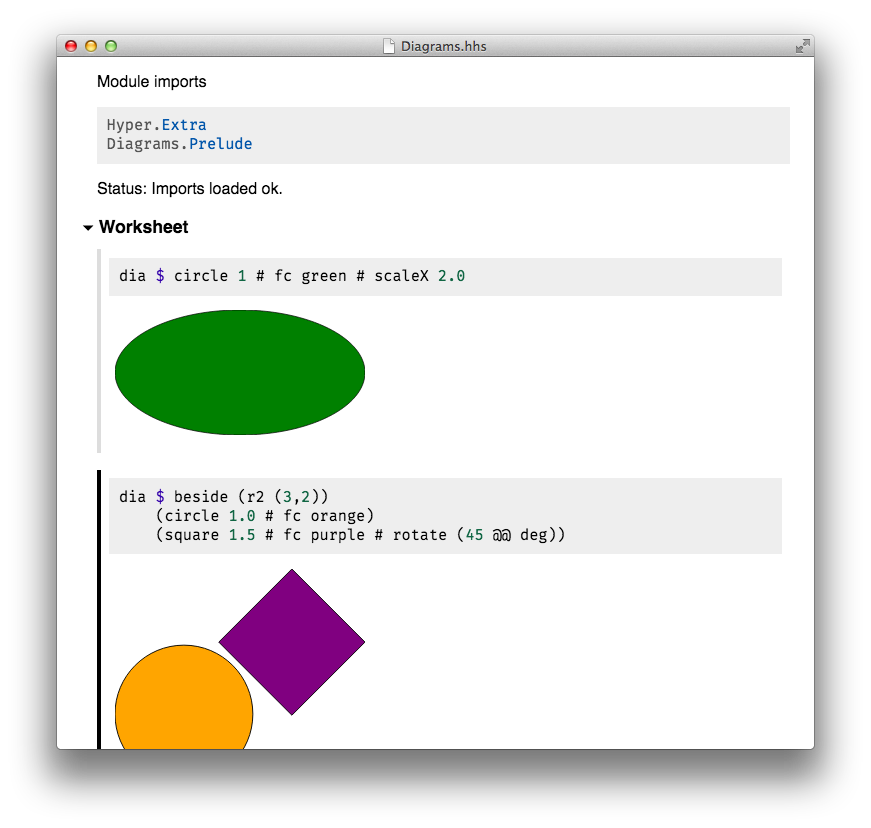
\includegraphics[width=\textwidth]{html/worksheet-diagrams.png}
\end{center}
%*endignore

\subsubsection*{Current status}

The very first release, \emph{Level $\alpha$}, version \verb`0.1.0.0` has been published. Basic features are working, but there is  plenty of room to grow. Please send me any feedback, suggestions, bug reports, contributions ... that you might have!

\subsubsection*{Future development}

Programming a computer usually involves writing a program text in a particular language, a ``verbal'' activity. But computers can also be instructed by gestures, say, a mouse click, which is a ``nonverbal'' activity. The long term goal of \emph{HyperHaskell} is to blur the lines between programming ``verbally'' and ``nonverbally'' in Haskell. This begins with an interpreter that has graphical representations for values, but also includes editing a program text while it's running (``live coding'') and interactive representations of values (e.g. ``tangible values''). This territory is still largely uncharted from a purely functional perspective, probably due to a lack of easily installed graphical facilities. It is my hope that \emph{HyperHaskell} may provide a common ground for exploration and experimentation in this direction, in particular by offering the \verb!Display! class which may, perhaps one day, replace our good old \verb!Show! class.

A simple form of live coding is planned for \emph{Level $\beta$}.

\FurtherReading
\begin{compactitem}
\item Project page and downloads: \url{https://github.com/HeinrichApfelmus/hyper-haskell}
\end{compactitem}
\end{hcarentry}
